\subsubsection{usergoal-ugMonitor}

\label{RE-use-case-ugMonitor}


the actCoordinator’s goal is to get the detailed list of existing crisis or alerts to decide on next actions
to undertake.		  


\begin{usecase}
  \addheading{Use-Case Description}
  \addsingletwocolumnrow{Name}{ugMonitor}
  \addsingletwocolumnrow{Scope}{system}
  \addsingletwocolumnrow{Level}{usergoal}
  

\addrowheading{Primary actor(s)}
\addnumberedsinglerow{}{\msrcode{actCoordinator[active]}}



\addrowheading{Goal(s) description}
\addsinglerow{the actCoordinator’s goal is to get the detailed list of existing crisis or alerts to decide on next actions
to undertake.}

\addrowheading{Reuse}
\addnumberedsinglerow{}{\msrucname{ugSecurelyUseSystem [1..1]}}
\addnumberedsinglerow{}{\msrucname{oeGetCrisisSet [1..*]}}
\addnumberedsinglerow{}{\msrucname{oeGetAlertSet [1..*]}}

\addrowheading{Protocol condition(s)}
\addnumberedsinglerow{}{the iCrash system has been deployed
}

\addrowheading{Pre-condition(s)}
\addnumberedsinglerow{}{
}

\addrowheading{Main post-condition(s)}
\addnumberedsinglerow{}{
}

\addrowheading{Main Steps}
\addalphanumberedsinglerow{}{the actor \msrcode{actCoordinator} executes the \msrucname{ugSecurelyUseSystem} use case}
\addalphanumberedsinglerow{}{the actor \msrcode{actCoordinator} executes the \msrucname{oeGetCrisisSet} use case}
\addalphanumberedsinglerow{}{the actor \msrcode{actCoordinator} executes the \msrucname{oeGetAlertSet} use case}
\addrowheading{Steps Ordering Constraints}
\addnumberedsinglerow{}{Step a must be executed before all other step}

\addrowheading{Additional Information}
\addsinglerow{
none
}

\end{usecase} 


Figure \ref{fig:lu.uni.lassy.excalibur.MyCrash.G02-RE-UCD-uc-ugMonitor}
shows how coordinators monitor crisis

\begin{figure}[htbp]
\begin{center}

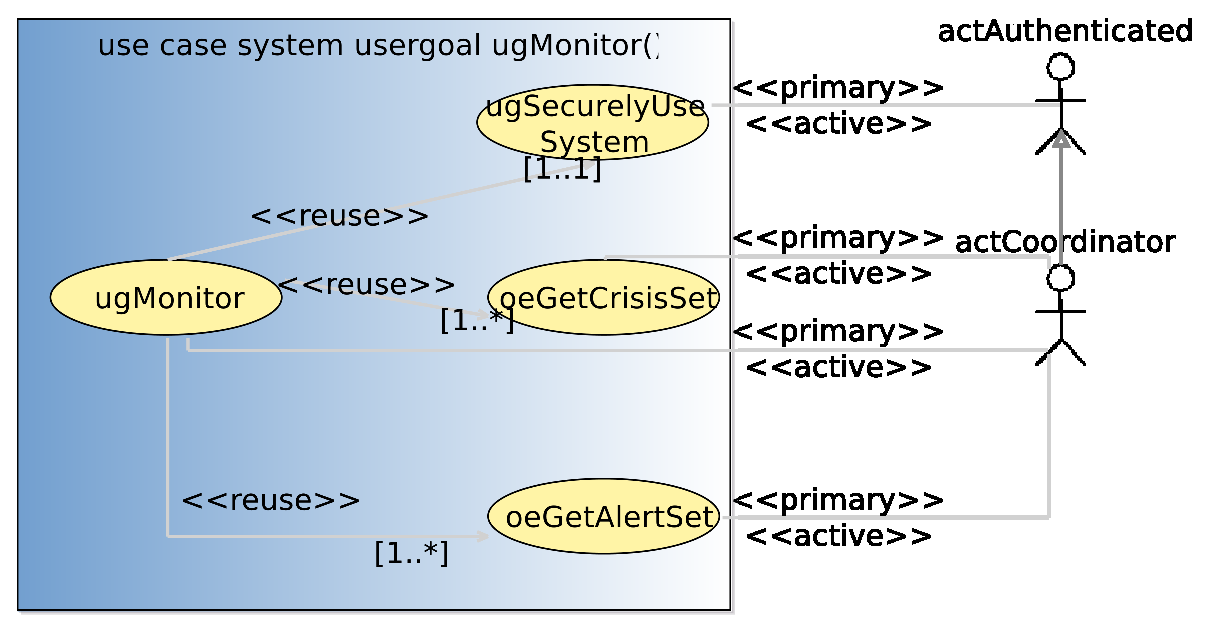
\includegraphics[
angle=0
]{./images-report-gen/usecase-model/usergoal/uc-ugMonitor.eps}
\end{center}
\caption[lu.uni.lassy.excalibur.MyCrash.G02 Use Case Diagram: uc-ugMonitor]{ugMonitor view}
\label{fig:lu.uni.lassy.excalibur.MyCrash.G02-RE-UCD-uc-ugMonitor}
\end{figure}
\vspace{0.5cm}
